% vim: ts=4 sts=4 sw=4 et tw=75
\chapter{Performance}
\label{chap:performance}
\begin{quote}
    His promises were, as he then was, mighty; But his performance, as he
    is now, nothing.
\end{quote}
\begin{quotesrc}
    Shakespeare, \bookname{King Henry VIII}
\end{quotesrc}

Long ago, programmers went to great effort to make their programs efficient
because computers were slow and expensive. Today, machines are much cheaper
and faster, so the need for absolute efficiency is greatly reduced. Is it
still worth worrying about performance?

Yes, but only if the problem is important, the program is genuinely too
slow, and there is some expectation that it can be made faster while
maintaining correctness, robustness, and clarity. A fast program that gets
the wrong answer doesn't save any time.

Thus the first principle of optimization is don't. Is the program good
enough already? Knowing how a program will be used and the environment it
runs in, is there any benefit to making it faster? Programs written for
assignments in a college class are never used again; speed rarely matters.
Nor will speed matter for most personal programs, occasional tools, test
frameworks, experiments, and prototypes. The run-time of a commercial
product or a central component such as a graphics library can be critically
important, however, so we need to understand how to think about performance
issues.

When should we try to speed up a program? How can we do so? What can we
expect to gain? This chapter discusses how to make programs run faster or
use less memory. Speed is usually the most important concern, so that is
mostly what we'll talk about. Space (main memory, disk) is less frequently
an issue but can be crucial, so we will spend some time and space on that
too.

As we observed in Chapter \ref{chap:alds}, the best strategy is to use the
simplest, cleanest algorithms and data structures appropriate for the task.
Then measure performance to see if changes are needed; enable compiler
options to generate the fastest possible code; assess what changes to the
program itself will have the most effect; make changes one at a time and
re-assess; and keep the simple versions for testing revisions against.

Measurement is a crucial component of performance improvement since
reasoning and intuition are fallible (易错的) guides and must be
supplemented with tools like timing commands and profilers (探查).
Performance improvement has much in common with testing, including such
techniques as automation, keeping careful records, and using regression
(回归) tests to make sure that changes preserve correctness and do not undo
previous improvements.

If you choose your algorithms wisely and write well originally you may find
no need for further speedups. Often minor changes will fix any performance
problems in well-designed code, while badly-designed code will require
major rewriting.

\section{A Bottleneck}
\label{sec:bootleneck}
Let us begin by describing how a bottleneck was removed from a critical
program in our local environment.

Our incoming mail funnels (漏斗) through a machine, called a gateway, that
connects our internal network with the external Internet. Electronic mail
messages from outside -- tens of thousands a day for a community of a few
thousand people -- arrive at the gateway and are transferred to the
internal network; this separation isolates our private network from the
public Internet and allows us to publish a single machine name (that of the
gateway) for everyone in the community.

One of the services of the gateway is to filter out "spam (罐头猪肉)."
unsolicited (未经同意的) mail that advertises services of dubious (可疑的)
merit (值得). After successful early trials of the spam filter, the service
was installed as a permanent feature for all users of the mail gateway, and
a problem immediately became apparent. The gateway machine, antiquated
(老旧的) and already very busy, was overwhelmed (倾覆) because the
filtering program was taking so much time -- much more time than was
required for all the other processing of each message -- that the mail
queues filled and message delivery was delayed by hours while the system
struggled to catch up.

This is an example of a true performance problem: the program was not fast
enough to do its job, and people were inconvenienced by the delay. The
program simply had to run much faster.

Simplifying quite a bit, the spam filter runs like this. Each incoming
message is treated as a single string, and a textual pattern matcher
examines that string to see if it contains any phrases from known spam,
such as "Make millions in your spare time" or "XXX-rated." Messages tend to
recur (重发), so this technique is remarkably effective, and if a spam
message is not caught, a phrase is added to the list to catch it next time.

None of the existing string-matching tools, such as \verb'grep', had the
right combination of performance and packaging (封装), so a special-purpose
spam filter was written. The original code was very simple; it looked to
see if each message contained any of the phrases (patterns):
\begin{wellcode}
    /* isspam: test mesg for occurrence of any pat */
    int isspam(char *mesg)
    {
        int i;

        for (i = 0; i < npat; i++)
            if (strstr(mesg, pat[i]) != NULL) {
                printf("spam: match for '%s'\n", pat[i]);
                return 1;
            }

        return 0;
    }
\end{wellcode}
How could this be made faster? The string must be searched, and the
\verb'strstr' function from the C library is the best way to search: it's
standard and efficient.

\emph{Using profiling (靠模切削),} a technique we'll talk about in the next
section, it became clear that the implementation of \verb'strstr' had
unfortunate properties when used in a spam filter. By changing the way
\verb'strstr' worked, it could be made more efficient \emph{for this
    particular problem}.

The existing implementation of \verb'strstr' looked something like this:
\begin{wellcode}
    /* simple strstr: use strchr to look for first character */
    char *strstr(const char *s1, const char *s2)
    {
        int n;

        n = strlen(s2);
        for (;;) {
            s1 = strchr(s1, s2[0]);
            if (s1 == NULL)
                return NULL;
            if (strncmp(s1, s2, n) == 0)
                return s1;
            s1++;
        }
    }
\end{wellcode}
It had been written with efficiency in mind, and in fact for typical use it
was fast because it used highly-optimized library routines to do the work.
It called \verb'strchr' to find the next occurrence of the first character
of the pattern, and then called \verb'strncmp' to see if the rest of the
string matched the rest of the pattern. Thus it skipped quickly over most
of the message looking for the first character of the pattern.  and then
did a fast scan to check the rest. Why would this perform badly?

There are several reasons. First, strncmp takes as an argument the length
of the pattern. which must be computed with \verb'strlen'. But the patterns
are fixed, so it shouldn't be necessary to recompute their lengths for each
message.

Second, \verb'strncmp' has a complex inner loop. It must not only compare
the bytes of the two strings, it must look for the terminating \verb'\0'
byte on both strings while also counting down the length parameter. Since
the lengths of all the strings are known in advance (though not to
strncmp), this complexity is unnecessary; we know the counts are right so
checking for the \verb'\n' wastes time.

Third, \verb'strchr' is also complex, since it must look for the character
and also watch for the \verb'\0' byte that terminates the message. For a
given call to \verb'isspam', the message is fixed, so time spent looking
for the \verb'\0' is wasted since we know where the message ends.

Finally, although \verb'strncmp', \verb'strchr' , and \verb'strlen' are all
efficient in isolation, the overhead of calling these functions is
comparable to the cost of the calculation they will perform. It's more
efficient to do all the work in a special, carefully written version of
\verb'strstr' and avoid calling other functions altogether.

These sorts of problems are a common source of performance trouble -- a
routine or interface works well for the typical case, but performs poorly
in an unusual case that happens to be central to the program at issue. The
existing \verb'strstr' was fine when both the pattern and the string were
short and changed each call, but when the string is long and fixed, the
overhead is prohibitive (可抑制的).

With this in mind, \verb'strstr' was rewritten to walk the pattern and
message strings together looking for matches, without calling subroutines.
The resulting implementation has predictable behavior: it is slightly
slower in some cases, but much faster in the spam filter and, most
important, is never terrible. To verify the new implementation's
correctness and performance, a performance test suite was built.  This
suite included not only simple examples like searching for a word in a
sentence, but also pathological (病态的) cases such as looking for a
pattern of a single x in a string of a thousand e's and a pattern of a
thousand x's in a string of a single e, both of which can be handled badly
by naive implementations. Such extreme cases are a key part of performance
evaluation.

The library was updated with the new \verb'strstr' and the spam filter ran
about $30\%$ faster, a good payoff for rewriting a single routine.

Unfortunately, it was still too slow.

When solving problems, it's important to ask right question. Up to now,
we've been asking for the fastest way to search for a textual pattern in a
string. But the real problem is to search for a large, fixed set of textual
patterns in a long, variable string. Put that way, \verb'strstr' is not so
obviously the right solution.

The most effective way to make a program faster is to use a better
algorithm.  With a clearer idea of the problem, it's time to think about
what algorithm would work best.

The basic loop,
\begin{wellcode}
    for (i = 0; i < npat; i++)
        if (strstr(mesg, pat[i]) != NULL)
            return 1;
\end{wellcode}
scans down the message \verb'npat' independent times; assuming it doesn't
find any matches, it examines each byte of the message \verb'npat' times,
for a total of \verb'strlen(mesg)*npat' comparisons.

A better approach is to invert the loops, scanning the message once in the
outer loop while searching for all the patterns in parallel in the inner loop:
\begin{wellcode}
    for (j = 0; mesg[j] != '\0'; j++)
        if (some pattern matches starting at mesg[j])
            return 1;
\end{wellcode}
The performance improvement stems from (主要来源于) a simple observation.
To see if any pattern matches the message at position \verb'j', we don't
need to look at all patterns, only those that begin with the same character
as \verb'mesg[j]'. Roughly, with 52 upper and lower-case letters we might
expect to do only \verb'strlen(mesg)*npat/52' comparisons. Since the
letters are not evenly distributed -- words with \verb's' more often than
\verb'x' -- we won't see a factor of 52 improvement, but we should see
some. In effect, we construct a hash table using the first character of the
pattern as the key.

Given some precomputation to construct a table of which patterns begin with
each character, \verb'isspam' is still short:
\begin{wellcode}
    int patlen[NPAT];                   /* length of pattern */
    int starting[UCHAR_MAX+1][NSTART];  /* pats starting with char */
    int nstarting[UCHAR_MAX+1];         /* number of such patterns */
    ...
    /* isspam: test mesg for occurrence of any pat */
    int isspam(char *mesg)
    {
        int i, j, k;
        unsigned char c;

        for (j = 0; (c = mesg[j]) != '\0'; j++) {
            for (i = 0; i < nstarting[c]; i++) {
                k = starting[c][i];
                if (memcmp(mesg+j, pat[k], patlen[k]) == 0) {
                    printf("spam: match for '%s'\n", pat[k]);
                    return 1;
                }
            }
        }
        return 0;
    }
\end{wellcode}
The two-dimensional array \verb'starting[c][]' stores, for each character
\verb'c', the indices of those patterns that begin with that character. Its
companion \verb'nstarting[c]' records how many patterns begin with
\verb'c'. Without these tables, the inner loop would run from 0 to
\verb'npat', about a thousand; instead it runs from 0 something like 20.
Finally, the array element \verb'patlen[k]' stores the precomputed result
of \verb'strlen(pat[k])'.

The following figure sketches (概括) these data structures for a set of
three pattern that begin with the letter \verb'b':
\begin{figure}[h]
\centering
\begin{varwidth}[t]{\textwidth}
    \vspace{0pt}
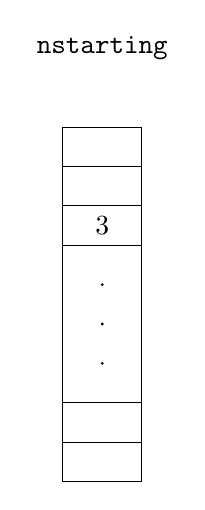
\begin{tikzpicture}
\draw (0, 0) -- (1, 0);
\draw (0, 4.5) -- (1, 4.5);
\draw (0, 0) -- (0, 4.5);
\draw (1, 0) -- (1, 4.5);

\draw (0, 3.0) -- (1, 3.0);
\draw (0, 3.5) -- (1, 3.5);
\draw (0, 4.0) -- (1, 4.0);
\node at (0.5, 3.25) {3};

\fill (0.5, 1.5) circle (0.02);
\fill (0.5, 2.0) circle (0.02);
\fill (0.5, 2.5) circle (0.02);

\draw (0, 0.5) -- (1, 0.5);
\draw (0, 1.0) -- (1, 1.0);

\node at (0.5, 5.5) {\texttt{nstarting}};
\end{tikzpicture}
\end{varwidth}
\qquad
\begin{varwidth}[t]{\textwidth}
    \vspace{0pt}
\begin{tikzpicture}
\draw (0, 0) -- (3, 0);
\draw (0, 4.5) -- (3, 4.5);
\draw (0, 0) -- (0, 4.5);
\draw (3, 0) -- (3, 4.5);

\draw (0, 3.5) -- (3, 3.5);
\draw (0, 3.0) -- (3, 3.0);

\draw (0.5, 3.0) -- (0.5, 3.5);
\draw (1.0, 3.0) -- (1.0, 3.5);
\draw (1.5, 3.0) -- (1.5, 3.5);
\node at (0.25, 3.25) {17};
\node at (0.75, 3.25) {35};
\node at (1.25, 3.25) {97};
\node at (-0.7, 3.25) {\verb"['b']"};

\node at (1.5, 5.5) {\texttt{starting}};
\end{tikzpicture}
\end{varwidth}
\qquad
\begin{varwidth}[t]{\textwidth}
    \vspace{0pt}
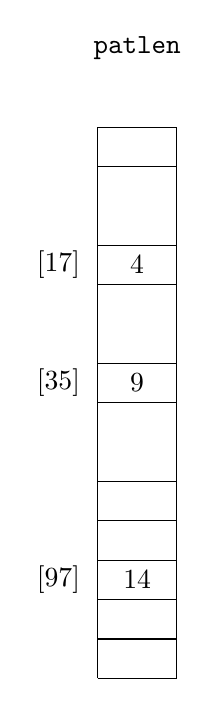
\begin{tikzpicture}
\foreach \y in {0.0, 0.5, 1.0, 1.5, 2.0, 2.5, 3.5, 4.0, 5.0, 5.5, 6.5,
	7.0} {
    \draw (0, \y) -- (1, \y);
}
\draw (0, 0) -- (0, 7.0);
\draw (1, 0) -- (1, 7.0);

\node at (0.5, 1.25) {14};
\node at (0.5, 3.75) {9};
\node at (0.5, 5.25) {4};
\node at (-0.5, 1.25) {[97]};
\node at (-0.5, 3.75) {[35]};
\node at (-0.5, 5.25) {[17]};

\node at (0.5, 8.0) {\texttt{patlen}};
\end{tikzpicture}
\end{varwidth}
\qquad
\begin{varwidth}[t]{\textwidth}
    \vspace{0pt}
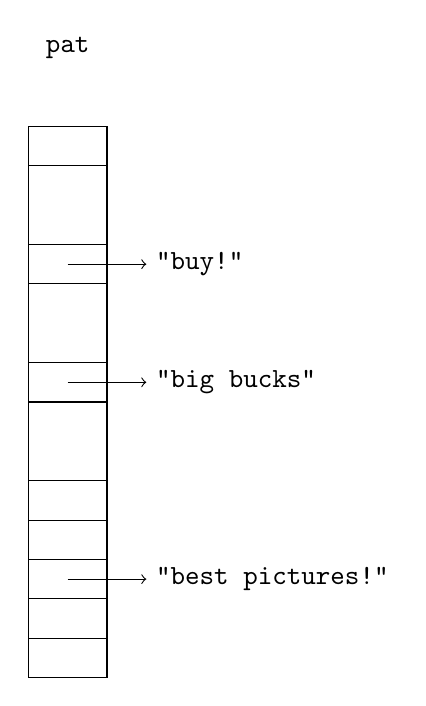
\begin{tikzpicture}
\foreach \y in {0.0, 0.5, 1.0, 1.5, 2.0, 2.5, 3.5, 4.0, 5.0, 5.5, 6.5,
	7.0} {
    \draw (0, \y) -- (1, \y);
}
\draw (0, 0) -- (0, 7.0);
\draw (1, 0) -- (1, 7.0);

\draw[->] (0.5, 1.25) -- (1.5, 1.25);
\draw[->] (0.5, 3.75) -- (1.5, 3.75);
\draw[->] (0.5, 5.25) -- (1.5, 5.25);
\node[right] at (1.5, 1.25) {\verb'"best pictures!"'};
\node[right] at (1.5, 3.75) {\verb'"big bucks"'};
\node[right] at (1.5, 5.25) {\verb'"buy!"'};

\node at (0.5, 8.0) {\texttt{pat}};
\end{tikzpicture}
\end{varwidth}

\end{figure}

The code to build these tables is easy:
\begin{wellcode}
    int i;
    unsigned char c;

    for (i = 0; i < npat; i++) {
        c = pat[i][0];
        if (nstarting[c] >= NSTART)
            printf("too many patterns (>=%d) begin '%c'",
                    NSTART, c);
        starting[c][nstarting[c]++] = i;
        patlen[i] = strlen(pat[i]);
    }
\end{wellcode}

Depending on the input, the spam filter is now five to ten times faster
than it was using the improved \verb'strstr', and seven to fifteen times
faster than the original implementation. We didn't get a factor of 52,
partly because of the non-uniform distribution of letters, partly because
the loop is more complicated in the new program, and partly because there
are still many failing string comparisons to execute, but the spam filter
is no longer the bottleneck for mail delivery. Performance problem solved.

The rest of this chapter will explore the techniques used to discover
performance problems, isolate the slow code. and speed it up. Before moving
on, though, it's worth looking back at the spam filter to see what lessons
it teaches. Most important, make sure performance matters. It wouldn't have
been worth all the effort if spam filtering wasn't a bottleneck. Once we
knew it was a problem, we used profiling and other techniques to study the
behavior and learn where the problem really lay. Then we made sure we were
solving the right problem, examining the overall program rather than just
focusing on \verb'strstr', the obvious but incorrect suspect. Finally, we
solved the correct problem using a better algorithm, and checked that it
really was faster. Once it was fast enough, we stopped; why over-engineer?

\begin{exercise}
    A table that maps a single character to the set of patterns that begin
    with that character gives an order of magnitude (巨大的) improvement.
    Implement a version of \verb'isspam' that uses two characters as the
    index. How much improvement does that lead to? These are simple special
    cases of a data structure called a trie. Most such data structures are
    based on trading (交易) space for time.
\end{exercise}

\section{Timing and Profiling}
\emph{Automate timing measurements.} Most systems have a command to measure
how long a program takes. On Unix, the command is called \verb'time':
\begin{wellcode}
    % time slowprogram
    real    7.0
    user    6.2
    sys     0.1
    %
\end{wellcode}
This runs the command and reports three numbers, all in seconds: "real"
time, the elapsed time for the program to complete; "user" CPU time, time
spent executing the user's program; and "system" CPU time, time spent
within the operating system on the program's behalf. If your system has a
similar command, use it; the numbers will be more informative, reliable,
and easier to track than time measured with a stopwatch. And keep good
notes. As you work on the program, making modifications and measurements,
you will accumulate a lot of data that can become confusing a day or two
later. (Which version was it that ran $20\%$ faster?) Many of the
techniques we discussed in the chapter on testing can be adapted for
measuring and improving performance. Use the machine to run and measure
your test suites and, most important, use regression (回归) testing to make
sure your modifications don't break the program.

If your system doesn't have a \verb'time' command, or if you're timing a
function in isolation, it's easy to construct a timing scaffold (脚手架)
analogous to a testing scaffold. C and C++ provide a standard routine,
clock, that reports how much CPU time the program has consumed so far. It
can be called before and after a function to measure CPU usage:
\begin{wellcode}
    #include <time.h>
    #include <stdio.h>
        ...
        clock_t before;
        double  elapsed;

        before = clock();
        long_running_function();
        elapsed = clock() - before;
        printf("function used %.3f seconds\n",
                elapsed / CLOCKS_PER_SEC);
\end{wellcode}
The scaling (定比) term, \verb'CLOCKS_PER_SEC', records the resolutions of the
timer as reported by clock. If the function takes only a small fraction of
a second, run it in a loop, but be sure to compensate (补偿) for loop
overhead if that is significant:
\begin{wellcode}
    before = clock();
    for (i = 0; i < 1000; i++)
        short_running_function();
    elapsed = (clock(0 - before) / (double)i;
\end{wellcode}
In Java, functions in the \verb'Date' class give wall clock time, which is
an approximation to CPU time:
\begin{wellcode}
    Date before = new Date();
    long_running_function();
    Date after = new Date();
    long elapsed = after.getTime() - before.getTime();
\end{wellcode}
The return value of \verb'getTime' is in milliseconds.

\emph{Use a profiler (刻画器).} Besides a reliable timing method, the most
important tool for performance analysis is a system for generating
profiles. A profile is a measurement of where a program spends its time.
Some profiles list each function, the number of times it is called, and the
fraction of execution time it consumes. Others show counts of how many
times each statement was executed. Statements that are executed frequently
contribute more to run-time, while statements that are never executed may
indicate useless code or code that is not being tested adequately.

Profiling is an effective tool for finding \textit{hot spots} in a program,
the functions or sections of code that consume most of the computing time.
Profiles should be interpreted with care, however. Given the sophistication
of compilers and the complexity of caching and memory effects, as well as
the fact that profiling a program affects its performance, the statistics
in a profile can be only approximate.

In the 1971 paper that introduced the term profiling, Don Knuth wrote that
"less than 4 percent of a program generally accounts for more than half of
its running time." This indicates that the way to use profiling is to
identify the critical time-consuming parts of the program, improve them to
the degree possible, and then measure again to see if a new hot spot has
surfaced. Eventually, often after only one or two iterations, there is no
obvious hot spot left.

Profiling is usually enabled with a special compiler flat or option. The
program is run, and then an analysis tool shows the results. On Unix, the
% XXX The hyperlink of footnote doesn't response when click.
flag is usually \verb'-p' and the tool is called
\verb"prof"\footnote{\texttt{gprof} in Linux}:
\begin{wellcode}
    % cc -p spamtest.c -o spamtest
    % spamtest
    % prof spamtest
\end{wellcode}
The following table shows the profile generated by a special version of the
spam filter we built to understand its behavior. It uses a fixed message
and a fixed set of 217 phrases, which it matches against the message
10000 times. This run on a 250 MHz MIPS R 10000 used the original
implementation of \verb'strstr' that calls other standard functions. The
output has been edited reformatted so it fits the page. Notice how sizes of
input (217 phrases) and the number of runs (10000) show up as consistency
checks in the "calls" column, which counts the number of calls of each
function.
\begin{wellcode}
    12234768552: Total number of instructions executed
    13961810001: Total computed cycles
    55.847: Total computed execution time (secs)
    1.141: Average cycles per instruction
\end{wellcode}
\begin{tabular}{rrrrrrr}
    secs    & \%    & cum\% & cycles    & instructions  & calls & function
    \\
    \hline
    \hline
    45.260  & 81.0\%    & 81.0\%    & 11314990000   & 9440110000    &
    48350000    & \verb'strchr' \\
    6.081   & 10.9\%    & 91.9\%    & 1520280000    & 1566460000    &
    46180000    & \verb'strncmp'    \\
    2.592   & 4.6\%     & 94.6\%    & 648080000     & 854500000     &
    2170000 & \verb'strstr' \\
    1.825   & 3.3\%     & 99.8\%    & 456225559     & 344882213     &
    21704435    & \verb'strlen' \\
    0.088   & 0.2\%     & 100.0\%   & 21950000      & 28510000      & 10000
    & \verb'isspam' \\
    0.000   & 0.0\%     & 100.0\%   & 100025    & 100028    & 1 &
    \verb'main'   \\
    0.000   & 0.0\%     & 100.0\%   & 53677     & 70268     & 219   &
    \verb'_memcopy' \\
    0.000   & 0.0\%     & 100.0\%   & 48888     & 46403     & 217   &
    \verb'strcpy'   \\
    0.000   & 0.0\%     & 100.0\%   & 17989     & 19894     & 219   &
    \verb'fgets'    \\
    0.000   & 0.0\%     & 100.0\%   & 16798     & 17547     & 230   &
    \verb'__malloc' \\
    0.000   & 0.0\%     & 100.0\%   & 10305     & 10900      & 204  &
    \verb'realfree' \\
    0.000   & 0.0\%     & 100.0\%   &  6293     & 7161      & 217   &
    \verb'estrdup'  \\
    0.000   & 0.0\%     & 100.0\%   & 6032      & 8575      & 231   &
    \verb'cleanfree'    \\
    0.000   & 0.0\%     & 100.0\%   & 5932      & 5729      & 1     &
    \verb'readpat'  \\
    0.000   & 0.0\%     & 100.0\%   & 5899      & 6339      & 219   &
    \verb'getline'  \\
    0.000   & 0.0\%     & 100.0\%   & 5500      & 5720      & 220   &
    \verb'_malloc'  \\
\end{tabular}

It's obvious that \verb'strchr' and \verb'strncmp', both called by
\verb'strstr', completely dominate the performance. Knuth's guideline is
right: a small part of the program consumes most of the run-time. When a
program is first profiled, it's common to see the top-running function at
50 percent or more, as it is here, making it easy to decide where to focus
attention.

\emph{Concentrate on the hot spots.} After rewriting \verb'strstr', we
profiled \verb'spamtest' again and found that 99.8\% of the time was now
spent in \verb'strstr' alone, even though the whole program was
considerable faster. When a single function is so overwhelmingly (压倒性的)
the bottleneck, there are only two ways to go: improve the function to use
a better algorithm, or eliminate the function altogether by rewriting the
surrounding program.

In this case, we rewrote the program. Here are the first few lines of the
profile for \verb'spamtest' using the final, fast implementation of
\verb'isspam'. Notice that the overall time is much less, that
\verb'memcmp' is now the hot spot, and that \verb'isspam' now consumes a
significant fraction of the computation. It is more complex than the
version that called \verb'strstr', but its cost is more than compensated
for by eliminating \verb'strlen' and \verb'strchr' from \verb'isspam' and
by replacing \verb'strncmp' with \verb'memcmp', which does less work per
byte.
\begin{tabular}{rrrrrrr}
    secs    & \%    & cum\% & cycles    & instructions  & calls & function
    \\
    \hline
    \hline
    3.524   & 56.9\%    & 56.9\%    & 880890000 & 1027590000    & 46180000
    & \verb'memcmp' \\
    2.662   & 43.04\%   & 100.0\%   & 665550000 & 902920000     & 10000
    & \verb'isspam' \\
    0.001   & 0.0\%     & 100.0\%   & 140304    & 106043        & 652
    & \verb'strlen' \\
    0.000   & 0.0\%     & 100.0\%   & 100025    & 100028        & 1
    & \verb'main'   \\
\end{tabular}

It's instructive (有益的) to spend some time comparing the cycle counts and
number of calls in the two profiles. Notice that \verb'strlen' went from a
couple of million calls to 652, and that strncmp and memcmp are called the
same number of times. Also notice that \verb'isspam'. which now
incorporates (吸收) the function of \verb'strchr', still manages to use far
fewer cycles than \verb'strchr' did before because it examines only the
relevant patterns at each step. Many more details of the execution can be
discovered by examining the numbers.

A hot spot can often be eliminated, or at least cooled, by much simpler
engineering than we undertook for the spam filter. Long ago, a profile of
Awk indicated that one function was begin called about a million times over
the course of a regression (回归) test, in this loop:
\begin{badcode}
    for (j = i; j < MAXFLD; j++)
        clear(j);
\end{badcode}
The loop, which clears fields before each new input line is read, was
taking as much as 50 percent of the run-time. The constant \verb'MAXFLD'.
the maximum number of fields permitted in an input line, was 200. But in
most uses of Awk, the actual number of fields was only two or three. Thus
an enormous amount of time was being wasted clearing fields that had never
been set. Replacing the constant by the previous value of the maximum
number of fields gave a 25 percent overall speedup. The fix was to change
the upper limit of the loop:
\begin{wellcode}
    for (j = i; j < maxfld; j++)
        clear(j);
    maxfld = i;
\end{wellcode}

\emph{Draw a picture.} Pictures are especially good for presentating
performance measurements. They can convey information about the effects of
parameter changes, compare algorithms and data structures, and sometimes
point to unexpected behavior. The graphs of chain length counts for several
hash multipliers in Chapter \ref{chap:debug} showed clearly  that some
multipliers were better than others.

% XXX The hyperlink of footnote doesn't response when click.
The following graph\footnote{Lack of graphs, because the graph is too
    blurry and ugly to represent.} shows the effect of the size of the hash
table array on run-time for the C version of \verb'markov' with Psalms as
input (42685 words, 22482 prefixes). We did two experiments. One set of
runs used array sizes that are powers of two from 2 to 16384; the other
used sizes that are the largest prime less than each power of two. We
wanted to see if a prime array size made any measurable difference to the
performance.

The graph shows that run-time for this input is not sensitive to the table
size once the size is above 1000 elements, nor is there a discernible
(可辨别的) difference between prime and power-of-two table sizes.

\begin{exercise}
    Whether or not your system has a \verb'time' command, use \verb'clock'
    or \verb'getTime' to write a timing facility for your own use. Compare
    its times t a wall clock. How does other activity on the machine affect
    the timing?
\end{exercise}
\begin{exercise}
    In the first profile, \verb'strchr' was called 48,350,000 times and
    \verb'strncmp' only 46,180,000. Explain the difference.
\end{exercise}

\section{Strategies for Speed}

Before changing a program to make it faster, be certain that it really is
too slow, and use timing tools and profilers to discover where the time is
going.  Once you know what's happening, there are a number of strategies to
follow. We list a few here in decreasing order of profitability (收益性).

\emph{Use a better algorithm or data structure.} The most important factor
in making a program faster is the choice of algorithm and data structure;
there can be a huge difference between an algorithm that is efficient and
one that is not. Our spam filter saw a change in data structure that was
worth a factor of ten; even greater improvement is possible if the new
algorithm reduces the order (阶数) of computation, say from $O(n^2)$ to
$O(n \log n)$. We covered this topic in Chapter \ref{chap:alds}, so we
won't dwell on (详述) it here.

Be sure that the complexity is really what you expect; if not, there might
be a hidden performance bug. This apparently linear algorithm for scanning
a string,
\begin{badcode}
    for (i = 0; i < strlen(s); i++)
        if (s[i] == c)
            ...
\end{badcode}
is in fact quadratic (平方的): if \verb's' has \verb'n' characters, each
call to \verb'strlen' walks down the \verb'n' characters of the string and
the loop is performed \verb'n' times.

\emph{Enable compiler optimizations.} One zero-cost change that usually
produces a reasonable improvement is to turn on whatever optimization the
compiler provides.  Modern compilers do sufficiently well that they obviate
(排除) much of the need for small-scale changes by programmers.

By default, most C and C++ compilers do not attempt much optimization. A
compiler option enables the optimizer ("improver" would be a more accurate
term). It should probably be the default except that the optimizations tend
to confuse source-level debuggers, so programmers must enable the optimizer
explicitly once they believe the program has been debugged.

Compiler optimization usually improves run-time anywhere from a few percent
to a factor of two. Sometimes, though, it slows the program down, so
measure the improvement before shipping (装运) your product. We compared
unoptimized and optimized compilation on a couple of versions of the spam
filter. For the test suite using the final version of the matching
algorithm, the original run-time was 8.1 seconds, which dropped to 5.9
seconds when optimization was enabled, an improvement of over 25\%. On the
other hand, the version that used the fixed-up \verb'strstr' showed no
improvement under optimization, because \verb'strstr' had already been
optimized when it was installed in the library; the optimizer applies only
to the source code being compiled now and not to the system libraries.
However, some compilers have global optimizer -- which analyze the entire
program for potential improvements. If such a compiler is available on your
system, try it; it might squeeze out a few more cycles.

One thing to be aware of is that the more aggressively the compiler
optimizes, the more likely it is to introduce bugs into the compiled
program. After enabling the optimizer, re-run your regression test suite,
as you should for any other modification.

\emph{Tune the code.} The right choice of algorithm matters if data sizes
are big enough. Furthermore, algorithmic improvements work across different
machines, compilers and languages. But once the right algorithm is in
place, if speed is still an issue the next thing to try is tuning the code:
adjusting the details of loops and expressions to make things go faster.

The version of \verb'isspam' we showed at the end of Section
\ref{sec:bootleneck} hadn't been tuned. Here, we'll show what further
improvements can be achieved by tweaking (扭) the loop. As a reminder, this
is how we left it:
\begin{wellcode}
    for (j = 0; (c = mesg[j]) != '\0'; j++) {
        for (i = 0; i < nstarting[c]; i++) {
            k = starting[c][i];
            if (memcmp(mesg+j, pat[k], patlen[k]) == 0) {
                printf("spam: match for '%s'\n", pat[k]);
                return 1;
            }
        }
    }
\end{wellcode}
This initial version takes 6.6 seconds in our test suite when compiled
using the optimizer. The inner loop has an array index
(\verb'nstarting[c]') in its loop condition whose value is fixed for each
iteration of the outer loop. We can avoid recalculating it by saving the
value in a local variable:
\begin{wellcode}
    for (j = 0; (c = mesg[j]) != '\0'; j++) {
        n = nstarting[c];
        for (i = 0; i < n; i++) {
            k = starting[c][i];
            ...
\end{wellcode}
This drops the time to 5.9 seconds, about 10\% faster, a speedup typical of
what tuning can achieve. There's another variable we can pull out:
\verb'starting[c]' is also fixed. It seems like pulling that computation
out of the loop would also help, but in our tests it made no measurable
difference. This, too, is typical of tuning: some things help, some things
don't, and one must measure to find out which. And results will vary with
different machines or compilers.

There is another change we could make to the spam filter. The inner loop
compares the entire pattern against the string, but the algorithm ensures
that the first character already matches. We can therefore tune the code to
start \verb'memcmp' one byte further along. We tried this and found it gave
about 3\% improvement, which is slight but it requires modifying only three
lines of the program, one of them in precomputation.

\emph{Don't optimize what doesn't matter.} Sometimes tuning achieves
nothing because it is applied where it makes no difference. Make sure the
code you're optimizing is where time is really spent. The following story
might be apocryphal (不可信的), but we'll tell it anyway. An early machine
from a now-defunct (现已倒闭的) company was analyzed with a hardware
performance monitor and discovered to be spending 50 percent of its time
executing the same sequence of several instructions. The engineers built a
special instruction to encapsulate the function of the sequence, rebuilt
the system, and found it made no difference at all; they had optimized the
idle loop of the operating system.

How much effort should you spend making a program run faster? The main
criterion (标准) is whether the changes will yield enough to be worthwhile.
As a guideline, the personal time spent making a program faster should not
be more than the time the speedup will recover during the lifetime of the
program. By this rule, the algorithmic improvement to \verb'isspam' was
worthwhile: it took a day of work but saved (and continues to save) hours
every day. Removing the array index from the inner loop was less dramatic
(戏剧性的) but still worth doing, since the program provides a service to a
large community. Optimizing public services like the spam filter or a
library is almost always worthwhile; speeding up test programs is almost
never worthwhile. And for a program that runs for a year, squeeze out
everything you can. It may be worth restarting if you find a way to make a
ten percent improvement even after the program has been running for a
month.

Competitive programs -- games, compilers. word processors, spreadsheets,
database systems -- fall into this category as well, since commercial
success is often to the swiftest, at least in published benchmark results.

It's important to time programs as changes are being made, to make sure
that things are improving. Sometimes two changes that each improve a
program will interact, negating (否定) their individual effects. It's also
the case that timing mechanisms can be so erratic (不稳定的) that it's hard
to draw firm conclusions about the effect of changes.  Even on single-user
systems,  times can fluctuate (波动) unpredictably. If the variability of
the internal timer (or at least what is reported back to you) is ten
percent, changes that yield improvements of only ten percent are hard to
distinguish from noise.

\section{Tuning the Code}

There are many techniques to reduce run-time when a hot spot is found. Here
are some suggestions, which should be applied with care, and with
regression testing after each to be sure that the code still works. Bear in
mind that good compilers will do some of these for you, and in fact you may
impede (阻止) their efforts by complicating the program. Whatever you try,
measure its effect to make sure it helps.

\emph{Collect common subexpressions.} If an expensive computation appears
multiple time, do it in only one place and remember the result. For
example, in Chapter \ref{chap:style} we showed a macro that computed a
distance by calling \verb'sqrt' twice in a row with the same values; in
effect the computation was
\begin{badcode}
    sqrt(dx*dx + dy*dy) + ((sqrt(dx*dx + dy*dy) > 0) ? ...)
\end{badcode}
Compute the square root once and use its value in two places.

If a computation is done within a loop but does not depend on anything that
changes within the loop, move the computation outside, as when we replaced
\begin{wellcode}
    for (i = 0; i < nstarting[c]; i++) {
\end{wellcode}
by
\begin{wellcode}
    n = nstarting[c];
    for (i = 0; i < n; i++) {
\end{wellcode}

\emph{Replace expensive operations by cheap ones.} The term
\textit{reduction in strength} refers to optimizations that replace an
expensive operation by a cheaper one. In olden times, this used to mean
replacing multiplications by additions or shifts, but that rarely buys much
now. Division and remainder are much slower than multiplication, however,
so there may be improvement if a division can be replaced with
multiplication by the inverse, or a remainder by a masking operation if the
divisor (除数) is a power of two.  Replacing array indexing by pointers in
C or C++ might speed things up, although most compilers do this
automatically. Replacing a function call by a simpler calculation can still
be worthwhile. Distance in the plane (平面) is determined by the formula
\verb'sqrt(dx*dx+dy*dy)', so to decide which of two points is further away
would normally involve calculating two square roots. But the same decision
can be made by comparing the squares of the distances:
\begin{wellcode}
    if (dx1*dx1 + dy1*dy1 < dx2*dx2 + dy2*dy2)
        ...
\end{wellcode}
gives the same result as comparing the square roots of the expressions.

Another instance occurs in textual pattern matchers such as our spam filter
or \verb'grep'. If the pattern begins with a literal character, a quick
search is made down the input text for that character; if no match is
found, the more expensive search machinery (结构)is not invoked at all.

\emph{Unroll (展开) or eliminate loops.} There is a certain overhead in
setting up and running a loop. If the body of the loop isn't too long and
doesn't iterate too many times, it can be more efficient to write out each
iteration in sequence. Thus, for example:
\begin{wellcode}
    for (i = 0; i < 3; i++)
        a[i] = b[i] + c[i];
\end{wellcode}
becomes
\begin{wellcode}
    a[0] = b[0] + c[0];
    a[1] = b[1] + c[1];
    a[2] = b[2] + c[2];
\end{wellcode}
This eliminates loop overhead, particularly branching, which can slow
modern processors by interrupting the flow of execution.

If the loop is longer, the same kind of transformation can be used to
amortize (分摊) the overhead over fewer iterations:
\begin{wellcode}
    for (i = 0; i < 3*n; i++)
        a[i] = b[i] + c[i];
\end{wellcode}
becomes
\begin{wellcode}
    for (i = 0; i < 3*n; i += 3) {
        a[i+0] = b[i+0] + c[i+0];
        a[i+1] = b[i+1] + c[i+1];
        a[i+2] = b[i+2] + c[i+2];
    }
\end{wellcode}
Note that this works only if the length is a multiple of the step size;
otherwise additional code is needed to fix up the ends, which is a place
for mistakes to creep in (潜入) and for some of the efficiency to be lost
again.

\emph{Cache frequently-used values.} Cached values don't have to be
recomputed.  Caching takes advantage of \textit{locality}, the tendency for
programs (and people) to re-use recently accessed or nearby items in
preference to (优先于) older or distant data. Computing hardware makes
extensive use of caches; indeed. adding cache memory to a computer can make
great improvements in how fast a machine appears. The same is true of
software.  Web browsers, for instance, cache pages and images to avoid the
slow transfer of data over the Internet. In a print preview program we
wrote years ago, non-alphabetic special characters like $\sfrac{1}{2}$ had
to be looked up in a table. Measurement showed that much of the use of
special characters involved drawing lines with long sequences of the same
single character. Caching just the single most recently used character made
the program significantly faster on typical inputs.

It's best if the caching operation is invisible from outside, so that it
doesn't affect the rest of the program except for making it run faster.
Thus in the case of the print previewer, the interface to the character
drawing function didn't change; it was always
\begin{wellcode}
    drawchar(c);
\end{wellcode}
The original version of \verb'drawchar' called \verb'show(lookup(c))'. The
cache implementation used internal static variables to remember the
previous character and its code:
\begin{wellcode}
    if (c != lastc) { /* update the cache */
        lastc = c;
        lastc = lookup(c);
    }
    show(lastc);
\end{wellcode}

\emph{Write a special-purpose allocator.} Often the single hot spot in a
program is memory allocation, which manifests (表明) itself as lots of
calls on \verb'malloc' or new. When most requests are for blocks of the
same size, substantial (实质的) speedups are possible by replacing calls to
the general-purpose allocator by calls to a special-purpose one.  The
special-purpose allocator makes one call to \verb'malloc' to fetch a big
array of items, then hands them out one at a time as needed, a cheaper
operation. Freed items are placed back in a free list so they can be reused
quickly.

If the requested sizes are similar, you can trade space for time by always
allocating enough for the largest request. This can be effective for
managing short strings if you use the same size for all strings up to a
specified length.

Some algorithms can use stack-based allocation, where a whole sequence of
allocations is done, and then the entire set is freed at once. The
allocator obtains one big chunk for itself and treats it as a stack,
pushing allocated items on as needed and popping them all off in a single
operation at the end. Some C libraries offer a function \verb'alloca' for
this kind of allocation, though it is not standard. It uses the local call
stack as the source of memory, and frees all the items when the function
that calls \verb'alloca' returns.

\emph{Buffer input and output.} Buffering batches transactions so that
frequent operations are done with as little overhead as possible, and the
high-overhead operations are done only when necessary. The cost of an
operation is thereby spread over multiple data values. When a C program
calls \verb'printf', for example, the characters are stored in a buffer but
not passed to the operating system until the buffer is full or flushed
explicitly. The operating system itself may in turn (轮流) delay writing
the data to disk. The drawback is the need to flush output buffers to make
data visible; in the worst case, information still in a buffer will be lost
if a program crashes.

\emph{Handle special cases separately.} By handling same-sized objects in
separate code, special-purpose allocators reduce time and space overhead in
the general allocator and incidentally (顺便) reduce fragmentation. In the
graphics library for the Inferno system, the basic draw function was
written to be as simple and straightforward as possible. With that working,
optimizations for a variety of cases (chosen by profiling) were added one
at a time; it was always possible to test the optimized version against the
simple one.  In the end, only a handful of cases were optimized because the
dynamic distribution of calls to the drawing function was heavily skewed
towards (为了) displaying characters; it wasn't worth writing clever code
for all the cases.

\emph{Precompute results.} Sometimes it is possible to make a program run
faster by precomputing values so they are ready when they are needed. We
saw this in the spam filter, which precomputed \verb'strlen(pat[i])' and
stored it in the array at \verb'patlen[i]'. If a graphics system needs to
repeatedly compute a mathematical function like sine but only for a
discrete (离散的) set of values, such as integer degrees, it will be faster
to precompute a table with 360 entries (or provide it as data) and index
into it as needed.  This is an example of trading space for time. There are
many opportunities to replace code by data or to do computation during
compilation, to save time and sometimes space as well. For example, the
\verb'ctype' functions like \verb'isdigit' are almost always implemented by
indexing into a table of bit flags rather than by evaluating a sequence of
tests.

\emph{Use approximate values.} If accuracy isn't an issue, use
lower-precision data types.  On older or smaller machines, or machines that
simulate floating point in software, single-precision floating-point
arithmetic is often faster than double-precision, so use \verb'float'
instead of \verb'double' to save time. Some modern graphics processors use
a related trick. The IEEE floating-point standard requires "graceful
underflow" as calculations approach the low end of representable values,
but this is expensive to compute. For images, the feature is unnecessary,
and it is faster and perfectly acceptable to truncate to zero. This not
only saves time when the numbers underflow, it can simplify the hardware
for all arithmetic. The use of integer \verb'sin' and \verb'cos' routines
is another example of using approximate values.

\emph{Rewrite in a lower-level language.} Lower-level languages tend to be
more efficient, although at a cost in programmer time. Thus rewriting some
critical part of a C++ or Java program in C or replacing an interpreted
script by a program in a compiled language may make it run much faster.

Occasionally, one can get significant speedups with machine-dependent code.
This is a last resort (手段), not a step to be taken lightly, because it
destroys portability and makes future maintenance and modifications much
harder.  Almost always, operations to be expressed in assembly language are
relatively small functions that should be embedded in a library;
\verb'memset' and \verb'memmove', or graphics operations, are typical
examples. The approach is to write the code as cleanly as possible in a
high-level language and make sure it's correct by testing it as we
described for \verb'memset' in Chapter \ref{chap:testing}.  This is your
portable version, which will work everywhere, albeit (虽然) slowly.  When
you move to a new environment, you can start with a version that is known
to work.  Now when you write an assembly-language version, test it
exhaustively (彻底地) against (针对) the portable one.  When bugs occur,
non-portable code is always suspect: it's comforting (令人鼓舞的) to have a
comparison implementation.

\begin{exercise}
    One way to make a function like \verb'memset' run faster is to have it
    write in word-sized chunks instead of byte-sized; this is likely to
    match the hardware better and might reduce the loop overhead by a
    factor of four or eight. The downside is that there are now a variety
    of end effects to deal with if the target is not aligned on a word
    boundary and if the length is not a multiple of the word size. Write a
    version of \verb'memset' that does this optimization. Compare its
    performance to the existing library version and to a straightforward
    byte-at-a-time loop.
\end{exercise}

\begin{exercise}
    Write a memory allocator \verb'smalloc' for C strings that uses a
    special-purpose allocator for small strings but calls \verb'malloc'
    directly for large ones. You will need to define a \verb'struct' to
    represent the strings in either case.  How do you decide where to
    switch from calling \verb'smalloc' to \verb'malloc'?
\end{exercise}

\section{Space Efficiency}

Memory used to be the most precious computing resource, always in short
supply, and much bad programming was done in an attempt to squeeze the most
out of what little there was. The infamous (声名狼藉的) "Year 2000 Problem"
is frequently cited as an example of this; when memory was truly scarce
(稀有), even the two bytes needed to store 19 were deemed (认为) too
expensive. Whether or not space is the true reason for the problem -- such
code may simply reflect the way people use dates in everyday life, where
the century is commonly omitted -- it demonstrates the danger inherent
(固有的) in short-sighted (短浅的) optimization.

In any case, times have changed, and both main memory and secondary storage
are amazingly cheap. Thus the first approach to optimizing space should be
the same as to improving speed: don't bother.

There are still situations, however, where space efficiency matters. If a
program doesn't fit into the available main memory, parts of it will be
paged out, and that will make its performance unacceptable. We see this
when new versions of software squander (使分散) memory; it is a sad reality
that software upgrades are often followed by the purchase of more memory.

\emph{Save space by using the smallest-possible data type.} One step to
space efficiency is to make minor changes to use existing memory better,
for example by using the smallest data type that will work. This might mean
replacing \verb'int' with \verb'short' if the data will fit; this is a
common technique for coordinates (协调) in 2-D graphics systems, since 16
bits are likely to handle any expected range of screen coordinates. Or it
might mean replacing \verb'double' with \verb'float'; the potential problem
is loss of precision, since \verb'float's usually hold only 6 or 7 decimal
digits.

In these cases and analogous ones, other changes may be required as well,
notably (特别是) format specifications in \texttt{printf} and especially
\texttt{scanf} statements.

The logical extension of this approach is to encode information in a byte
or even fewer bits, say a single bit where possible. Don't use C or C++
bit-fields; they are highly non-portable and tend to generate voluminous
(长篇的) and inefficient code.  Instead, encapsulate the operations you
want in functions that fetch and set individual bits within words or an
array of words with shift and mask operations. This function returns a
group of contiguous bits from the middle of a word:
\begin{wellcode}
    /* getbits: get n bits from position p */
    /* bits are numbered from 0 (least significant) up */
    unsigned int getbits(unsigned int x, int p, int n)
    {
        return (x >> (p+1-n)) & ~(~0 << n);
    }
\end{wellcode}
If such functions turn out to be too slow, they can be improved with the
techniques described earlier in this chapter. In C++, operator overloading
can be used to make bit accesses look like regular subscripting.

\emph{Don't store what you can easily recompute.} Changes like these are
minor, however; they are analogous to code tuning. Major improvements are
more likely to come from better data structures, perhaps coupled with
algorithm changes. Here's an example.  Many years ago, one of us was
approached (商量) by a colleague who was trying to do a computation on a
matrix so large that it was necessary to shut down the machine and reload a
stripped-down (精简的) operating system so the matrix would fit. He wanted
to know if there was an alternative, since this was an operational
nightmare. We asked what the matrix was like, and learned that it contained
integer values, \textit{most of which were zero.} In fact, fewer than five
percent of the matrix elements were non-zero. This immediately suggested a
representation in which only the non-zero elements of the matrix were
stored, and each matrix access like \verb'm[i][j]' would be replaced by a
function call \verb'm(i,j)'. There are several ways to store the data; the
easiest is probably an array of pointers, one for each row, each of which
points to a compact array of column numbers and corresponding values. This
has higher space overhead per non-zero item but requires much less space
overall, and although individual accesses will be slower, they will be
noticeably faster than reloading the operating system.  To complete the
story: the colleague applied the suggestion and went away completely
satisfied.

We used a similar approach to solve a modern version of the same problem. A
radio design system needed to represent terrain (地形) and radio signal
strengths over a very large geographical area (100 to 200 kilometers on a
side) to a resolution of 100 meters. Storing this as a large rectangular
array exceeded the memory available on the target machine and would have
caused unacceptable paging behavior. But over large regions, the terrain
and signal strength values are likely to be the same, so a hierarchical
representation that coalesces (联合) regions of the same value into a
single cell makes the problem manageable.

Variations on this theme are frequent, and so are specific representations,
but all share the same basic idea: store the common value or values
implicitly or in a compact form, and spend more time and space on the
remaining values. If the most common values are really common, this is a
win.

The program should be organized so that the specific data representation of
complex types is hidden in a class or set of functions operating on a
private data type.  This precaution (预防措施) ensures that the rest of the
program will not be affected if the representation changes.

Space efficiency concerns sometimes manifest (表现) themselves in the
external representation of information as well, both conversion (转换) and
storage. In general, it is best to store information as text wherever
feasible rather than in some binary representation.  Text is portable, easy
to read, and amenable (服从的) to processing by all kinds of tools; binary
representations have none of these advantages. The argument in favor of
binary is usually based on "speed," but this should be treated with some
skepticism (批判思想), since the disparity (差异) between text and binary
forms may not be all that great.

Space efficiency often comes with a cost in run-time. One application had
to transfer a big image from one program to another. Images in a simple
format called PPM were typically a megabyte, so we thought it would be much
faster to encode them for transfer in the compressed GIF format instead;
those files were more like 50K bytes. But the encoding and decoding of GIF
took as much time as was saved by transferring a shorter file, so nothing
was gained. The code to handle the GIF format is about 500 lines long; the
PPM source is about 10 lines. For ease of maintenance, therefore, the GIF
encoding was dropped and the application continues to use PPM exclusively.
Of course the tradeoff would be different if the file were to be sent
across a slow network instead; then a GIF encoding would be much more
cost-effective.

\section{Estimation}
\label{sec:estimation}

It's hard to estimate ahead of time how fast a program will be, and it's
doubly hard to estimate the cost of specific language statements or machine
instructions. It's easy, though, to create a cost model for a language or a
system, which will give you at least a rough idea of how long a important
operations take.

One approach that is often used for conventional programming languages is a
program that times representative code sequences. There are operational
difficulties, like getting reproducible results and canceling out
irrelevant overheads, but it is possible to get useful insights without
much effort. For example, we have a C and C++ cost model program that
estimates the costs of individual statements by enclosing them in a loop
that runs them many millions of times, then computes an average time. On a
250 MHz MIPS R10000, it produces this data, with times in nanoseconds per
operation.
\begin{wellcode}
    int operations:
        i1++                    8
        i1 = i2 + i3           12
        i1 = i2 - i3           12
        i1 = i2 * i3           12
        i1 = i2 / i3          114
        i1 = i2 % i3          114

    float operations
        f1 = f2                 8
        f1 = f2 + f3           12
        f1 = f2 - f3           12
        f1 = f2 * f3           11
        f1 = f2 / f3           28

    double operations
        d1 = d2                 8
        d1 = d2 + d3           12
        d1 = d2 - d3           12
        d1 = d2 * d3           11
        d1 = d2 / d3           58

    numeric conversions
        i1 = f1                 8
        f1 = i1                 8
\end{wellcode}
Integer operations are fast, except for division and modulus (取模).
Floating-point operations are as fast or faster, a surprise to people who
grew up at a time when floating point operations were much more expensive
than integer operations.

Other basic operations are also quite fast, including function calls, the
last three lines of this group:
\begin{wellcode}
    integer vector operations
        v[i] = i               49
        v[v[i]] = i            81
        v[v[v[i]]] = i        100

    control structures
        if (i == 5) i1++        4
        if (i != 5) i1++       12
        while (i < 0) i1++      3
        i1 = sum1(i2)          57
        i1 = sum2(i2, i3)      58
        i1 = sum3(i2, i3, i4)  54
\end{wellcode}
But input and output are not so cheap, nor are most other library function:
\begin{wellcode}
    input/output
        fputs(s, fp)                        270
        fgets(s, 9, fp)                     222
        fprintf(fp, "%d\n", i)             1820
        fscanf(fp, "%d", &i1)              2070

    malloc
        free(malloc(8))                     342

    string functions
        strcpy(s, "0123456789")             157
        i1 = strcmp(s, s)                   176
        i1 = strcmp(s, "a123456789")         64

    string/number conversions
        i1 = atoi("12345")                  402
        sscanf("12345", "%d", &i1)         2376
        sprintf(s, "%d", i)                1492
        f1 = atof("123.45")                4098
        sscanf("123.45", "%f", &f1)        6438
        sprintf(s, "%6.2f", 123.45)        3902
\end{wellcode}
The time for \verb'malloc' and \verb'free' are probably not indicative of
true performance, since freeing immediately after allocating is not a
typical pattern.

Finally, math functions:
\begin{wellcode}
    math functions
        i1 = rand()             135
        f1 = log(f2)            418
        f1 = exp(f2)            462
        f1 = sin(f2)            514
        f1 = sqrt(f2)           112
\end{wellcode}

These values would be different on different hardware, of course, but the
trends can be used for back-of-the-envelope (粗略) estimates of how long
something might take, or for comparing the relative costs of I/O versus
basic operations, or for deciding whether to rewrite an expression or use
an inline function.

There are many sources of variability. One is compiler optimization level.
Modern compilers can find optimizations that elude most programmers.
Furthermore, current CPUs are so complicated that only a good compiler can
take advantage of their ability to issue multiple instructions
concurrently, pipeline their execution, fetch instructions and data before
they are needed, and the like.

Computer architecture itself is another major reason why performance
numbers are hard to predict. Memory caches make a great difference in
speed, and much cleverness in hardware design goes into hiding the fact
that main memory is quite a bit slower than cache memory. Raw processor
clock rates (频率) like "400 MHz" are suggestive (提示性的) but don't tell
the whole story; one of our old 200 MHz Pentium is significantly slower
than an even older 100 MHz Pentium because the latter has a big
second-level cache and the former has none. And different generations of
processor, even for the same instruction set, take different numbers of
clock cycles to do a particular operation.

\begin{exercise}
    Create a set of tests for estimating the costs of basic operations for
    computers and compilers near you, and investigates and differences in
    performance.
\end{exercise}

\begin{exercise}
    Create a cost model for higher-level operations in C++. Among the
    features that might be included are construction, copying, and deletion
    of class objects; member function calls; virtual functions; inline
    functions; the \verb'iostream' library; the STL. This exercise is
    open-ended (开放式的), so Concentrate on a small set of representative
    operations.
\end{exercise}

\begin{exercise}
    Repeat the previous exercise for Java.
\end{exercise}
